% ============================================================================
% Laporan Sistem ENYX-Smart Hub
%
% KOMPILASI (terverifikasi 10 Oktober 2026):
%   cd docs && pdflatex laporan.tex && pdflatex laporan.tex   -> laporan.pdf (15 hal)
%
% Catatan compiler:
% - pdflatex (rekomendasi, termasuk recipe "pdfLaTeX" di VS Code LaTeX Workshop):
%   memilih figure .png secara otomatis (include ditulis tanpa ekstensi).
% - dvilualatex: dokumen juga compile menjadi DVI (memilih figure .eps),
%   namun konversi DVI -> PDF pada route dvipdfmx TIDAK mendukung EPS tanpa
%   Ghostscript. Pakai recipe pdfLaTeX untuk output PDF.
%
% Paket: geometry, graphicx, booktabs, longtable, array, xcolor, hyperref,
%        mathptmx (font Times New Roman / URW Nimbus Roman, ukuran 12pt)
%        (semua tersedia di TeX Live 2023/Debian: texlive-latex-base,
%         texlive-latex-recommended, texlive-fonts-recommended)
% Sumber diagram: docs/DIAGRAM.md (PlantUML) -> docs/figures/ (png + eps)
% ============================================================================
\documentclass[12pt,a4paper]{article}

\usepackage[utf8]{inputenc}
\usepackage[T1]{fontenc}
\usepackage{mathptmx}   % Times New Roman (URW Nimbus Roman) untuk teks & matematika
\usepackage[vmargin=2.2cm,hmargin=2.4cm]{geometry}
\usepackage{graphicx}
\usepackage{booktabs}
\usepackage{longtable}
\usepackage{array}
\usepackage{xcolor}
\usepackage[hidelinks]{hyperref}

\graphicspath{{figures/}{./}}

\setlength{\emergencystretch}{3em}   % kurangi overfull pada paragraf justified

\definecolor{enyxgreen}{HTML}{166534}
\definecolor{enyxlight}{HTML}{EAF4FB}
\definecolor{rowgray}{HTML}{F3F4F6}

\title{%
  \textbf{Laporan Sistem ENYX-Smart Hub}\\[6pt]
  \large Tata Kelola Pengemasan Kentang Berbasis IoT\\ dengan Traceability GS1 Digital Link%
}
\author{ENYX-Smart Hub --- Tim Pengembangan}
\date{Versi 2.0 --- 10 Oktober 2026}

\begin{document}

\maketitle

\begin{abstract}
\noindent
Laporan ini mendokumentasikan rancangan dan keputusan desain sistem ENYX-Smart Hub:
platform pengemasan kentang berbasis IoT yang mengintegrasikan timbangan RS485, scanner
barcode, printer label, dan MQTT broker pada satu server lokal dengan akses enterprise
melalui domain HTTPS. Laporan ini merupakan konsolidasi dari seluruh dokumen rancangan
sebelumnya (arsitektur, tech stack, perangkat keras, API, UI/UX, dan rencana implementasi)
ke dalam satu acuan resmi. Workflow, diagram arsitektur, dan skema database tetap dikelola
secara visual pada \texttt{docs/DIAGRAM.md}.
\end{abstract}

\tableofcontents
\newpage

% ============================================================================
\section{Pendahuluan}
% ============================================================================

\subsection{Latar Belakang}
Rantai pasok kentang di Indonesia umumnya masih bertumpu pada pencatatan manual pada
tahap pascapanen: penimbangan, sortir, hingga pengemasan sering dicatat di kertas atau
tidak dicatat sama sekali. Akibatnya, penelusuran asal produk (traceability) menjadi
lambat, data kesepakatan berat antara petani dan fasilitas mudah berbeda, dan produk
kesulitan memenuhi persyaratan ekspor yang menuntut identitas produk berstandar GS1.

ENYX-Smart Hub hadir untuk mendigitalkan alur tersebut end-to-end: mulai dari petani
menyerahkan hasil panen, operator memverifikasi dan menimbang, sortir grade, pengepakan
pouch 1 kg, penyimpanan warehouse, hingga pengiriman ekspor --- dengan pencatatan
otomatis di setiap tahap dan label berstandar GS1 (QR GS1 Digital Link, EAN-13, ITF-14).

\subsection{Tujuan Laporan}
\begin{itemize}
  \item Menjadi acuan tunggal (single reference) untuk desain sistem.
  \item Merekam keputusan desain beserta alasannya agar konsisten saat implementasi.
  \item Menjadi dasar assessment kelayakan teknis, biaya (BOM), dan rencana pengembangan.
\end{itemize}

\subsection{Lingkup Saat Ini}
Sistem beroperasi untuk \textbf{satu komoditas: Kentang} (grade A/B/C). Arsitektur dan
skema data dirancang \emph{multi-commodity-ready} sehingga penambahan komoditas baru
(Tomat, Cabai, dsb.) di masa depan hanya memerlukan data master tanpa migrasi skema.

% ============================================================================
\section{Keputusan Desain}

Tabel berikut merangkum keputusan desain final beserta alasannya. Keputusan ini
merefleksikan workflow operasional yang telah divalidasi pada \texttt{docs/DIAGRAM.md}.

\begin{longtable}{@{}>{\raggedright\arraybackslash}p{4.6cm}>{\raggedright\arraybackslash}p{6.2cm}>{\raggedright\arraybackslash}p{4.6cm}@{}}
\toprule
\textbf{Keputusan} & \textbf{Alasan} & \textbf{Dampak} \\
\midrule
\endhead
Satu komoditas: Kentang & Fokus MVP, operasional tunggal; multi-commodity belum jadi kebutuhan & Kolom \texttt{commodityId} tetap ada; kode commodity \texttt{002}/\texttt{003} reserved \\
\hline
Petani hanya menunjukkan ID; \textbf{operator yang approve} berat & Menghindari sengketa di timbangan sekaligus menjaga interaksi petani tetap minimal & Status \texttt{APPROVED} dicatat operator; tidak ada aksi approval dari petani \\
\hline
Penimbangan hanya di Area Penerimaan (karung/palet) dan Area Pengepakan (pouch 1 kg) & Area Sortir tidak perlu timbangan; berat per grade diperoleh dari jumlah pouch & Timbangan dipindah/terbatas di 2 area; Area Sortir hanya cetak label grade \\
\hline
Pengepakan hanya melabeli, tanpa scan & Grade sudah terpisah dan berlabel pada palet & Scan manual di pengepakan dihilangkan; commodity/grade/pallet otomatis dari context \\
\hline
Palet dibuat saat scan pertama & Palet adalah unit fisik ber-ID dasar seluruh traceability & Entity \texttt{Pallet} dibuat saat penerimaan; kode \texttt{PLT-YYYYMMDD-SEQ} \\
\hline
Tanggal panen diinput operator saat penerimaan & Atribut wajib untuk traceability yang sebelumnya belum tertangkap & Field \texttt{harvestDate} pada entity \texttt{Pallet} \\
\hline
Label pouch memakai QR \textbf{GS1 Digital Link} & Satu simbol untuk dua pembaca: scanner internal dan smartphone konsumen; searah dengan arah industri (Sunrise 2027) & QR pouch berisi URL; server menyediakan resolver + halaman traceability publik; EAN-13 tetap dicetak paralel \\
\hline
Arsitektur centralized DB (bukan blockchain) & Fasilitas adalah aktor tunggal; database lokal terpercaya sudah cukup & Tanpa infra multi-pihak; blockchain ditunda sampai ada jaringan pemangku kepentingan \\
\bottomrule
\end{longtable}

% ============================================================================
\section{Arsitektur Sistem}

\subsection{Gambaran 5 Layer}
Sistem disusun dalam lima layer, dari perangkat lapangan hingga akses pengguna:

\begin{longtable}{@{}>{\raggedright\arraybackslash}p{3.2cm}>{\raggedright\arraybackslash}p{7.0cm}>{\raggedright\arraybackslash}p{5.0cm}@{}}
\toprule
\textbf{Layer} & \textbf{Komponen} & \textbf{Fungsi} \\
\midrule
\endhead
Field Level & Timbangan RS485 (Area Penerimaan \& Pengemasan), scanner QR, printer label (palet, grade, pouch), scanner warehouse, scanner pengiriman, smartphone petani & Input data timbang, scan, dan cetak label di lapangan \\
\hline
Edge / Gateway & 2$\times$ ESP32 (Area Penerimaan, Area Pengemasan), router/switch & Akuisisi data timbangan via RS485; publish ke broker via MQTT/Wi-Fi LAN \\
\hline
Application Level & PC Server: web server (Nginx), aplikasi (business logic), MQTT broker (Mosquitto), session context manager, traceability page + GS1 Digital Link resolver, database & Logika bisnis, session context, penyajian halaman traceability, penyimpanan lokal \\
\hline
Cloud Level & Cloud database (Neon/Supabase) & Backup berkala dan disaster recovery \\
\hline
Enterprise Level & Domain HTTPS (Cloudflare + Let's Encrypt), akses pengguna & Akses admin/operator/petani dan halaman traceability publik untuk konsumen/buyer \\
\bottomrule
\end{longtable}

\begin{figure}[htbp]
  \centering
  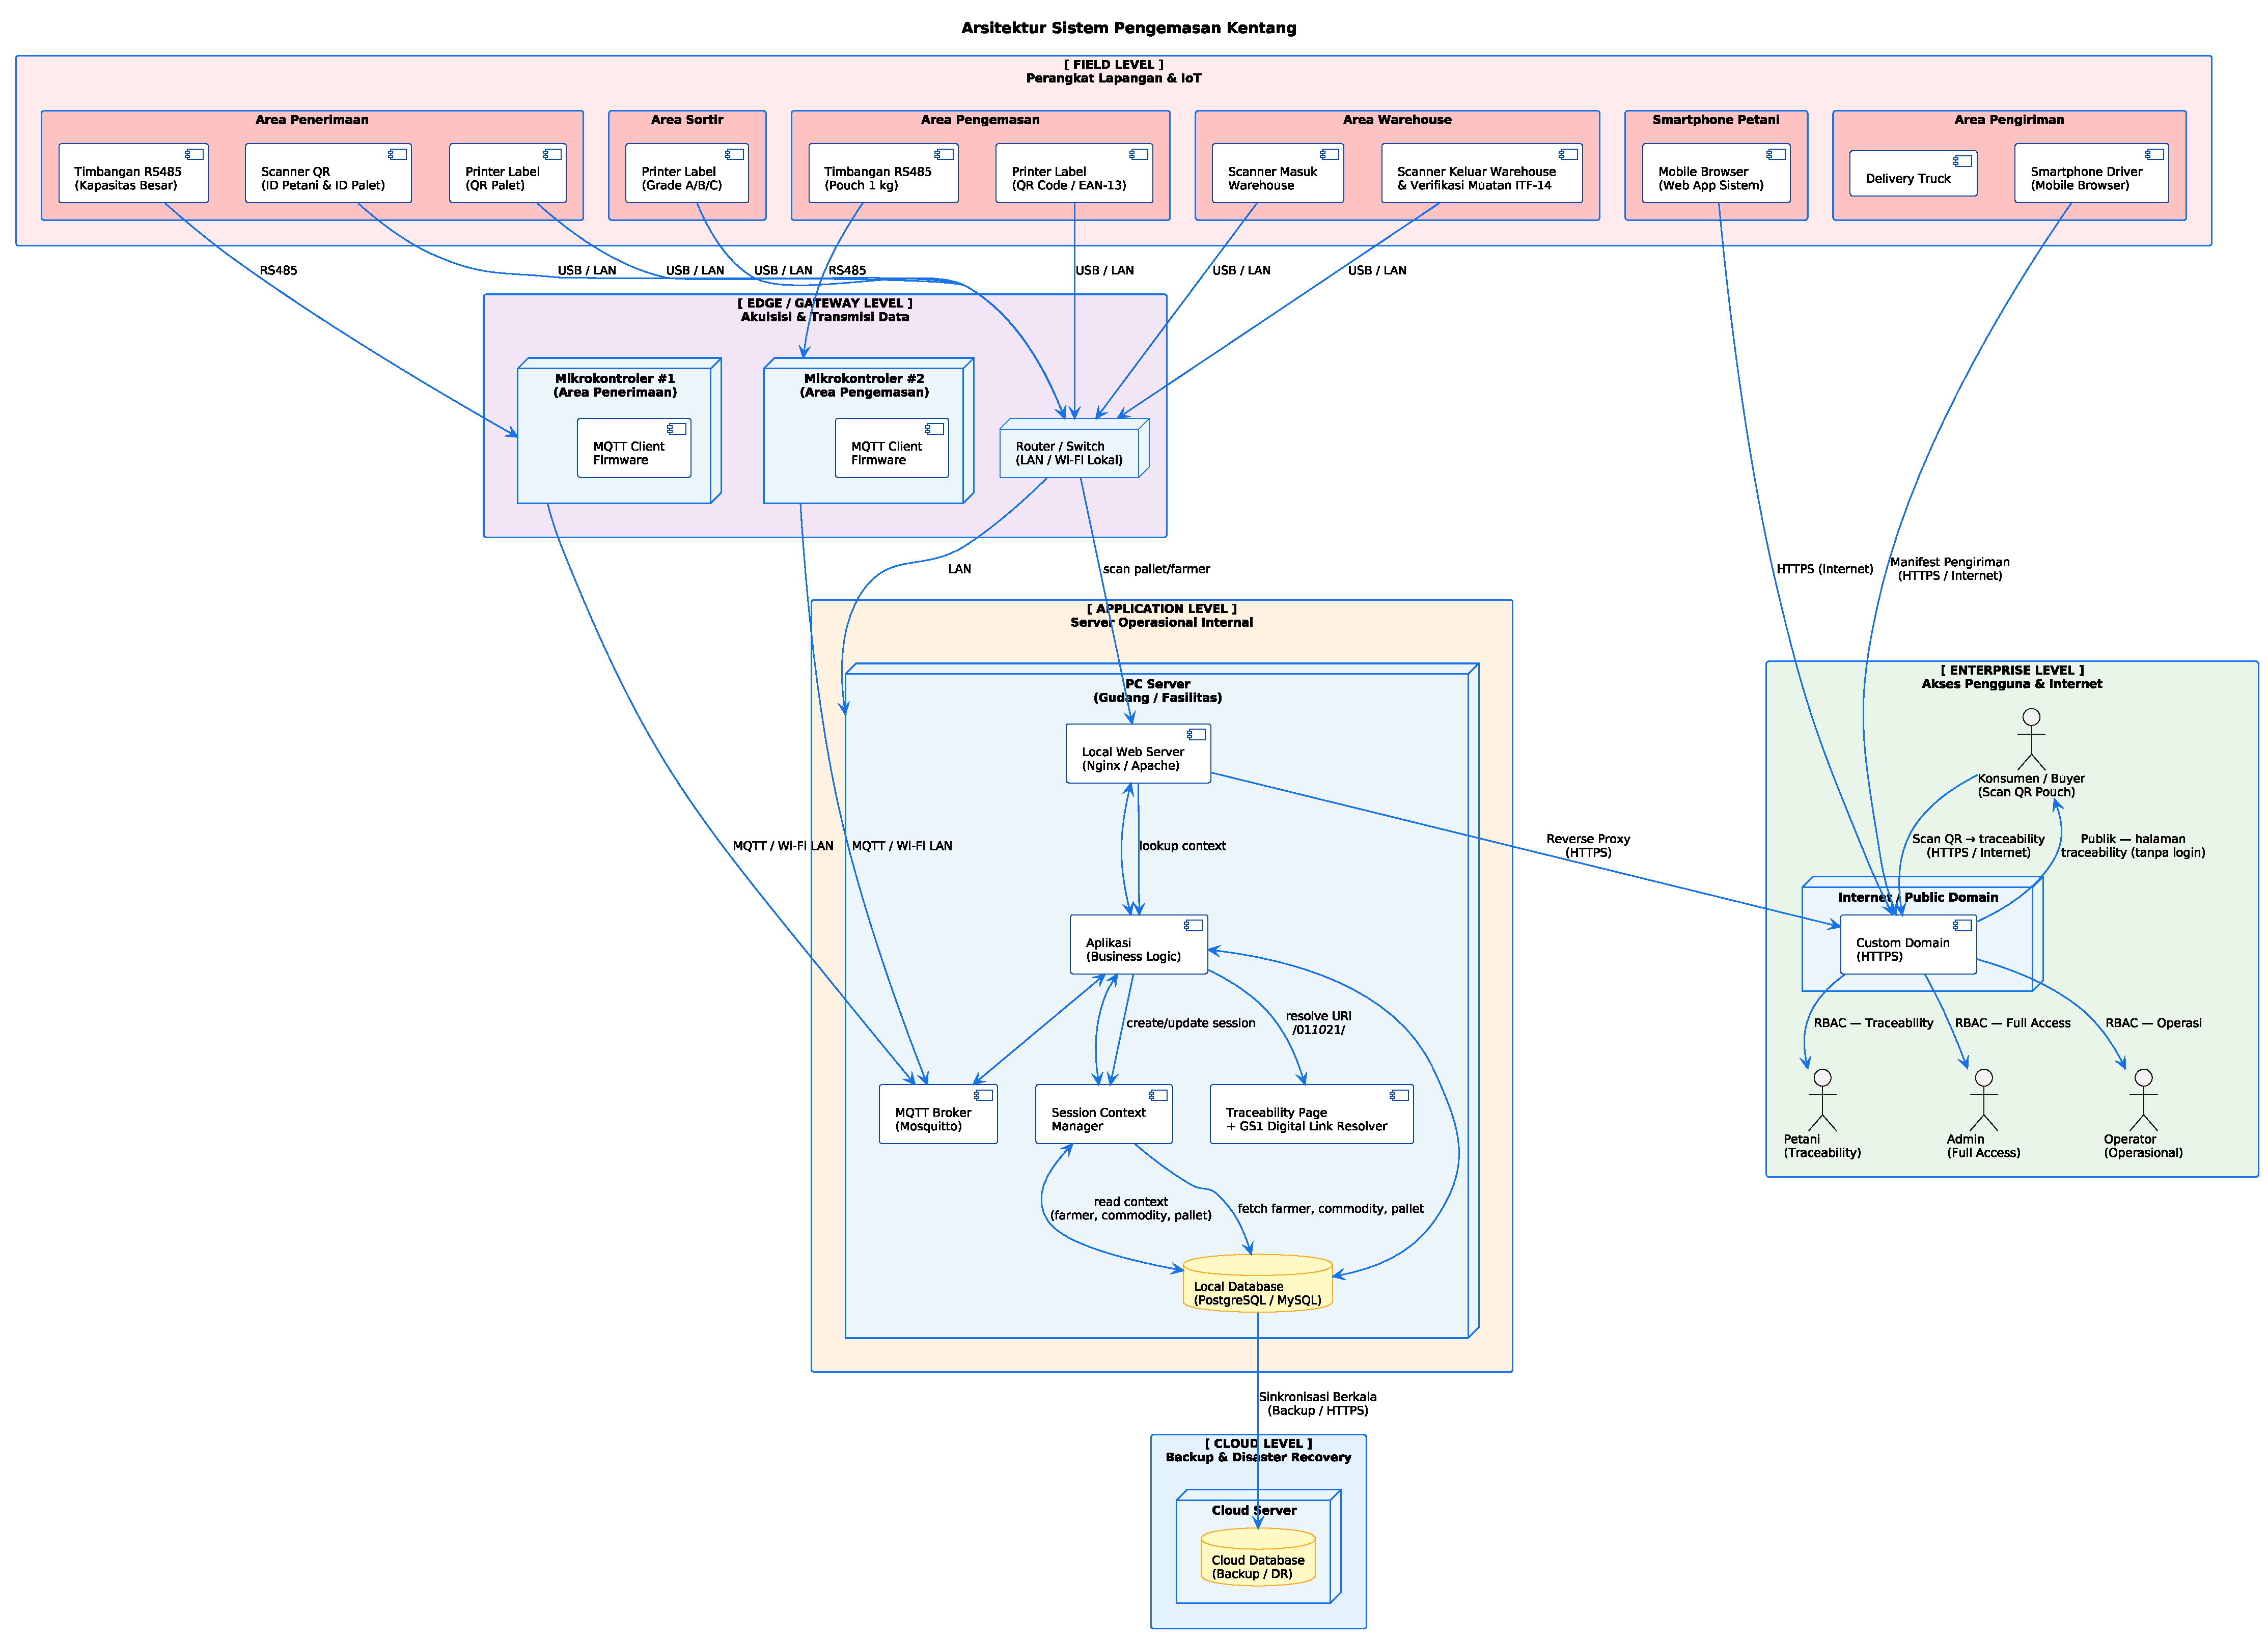
\includegraphics[width=\textwidth]{arsitektur}
  \caption{Diagram arsitektur sistem --- Field Level hingga Enterprise Level.\newline
  (Sumber: \texttt{docs/DIAGRAM.md}; render terakhir 10 Oktober 2026)}
\end{figure}

\subsection{Prinsip Deployment}
\begin{itemize}
  \item \textbf{Local-first}: seluruh layanan inti (backend, DB, broker, web) berjalan pada satu PC server di lokasi fasilitas; operasional tetap berjalan saat internet terputus.
  \item \textbf{Backup berkala}: sinkronisasi logis ke cloud database setiap 1--6 jam (cron/backup); data time-series diagregasi sebelum dikirim untuk menghemat bandwidth.
  \item \textbf{Keamanan}: HTTPS wajib untuk akses enterprise (Let's Encrypt); MQTT broker memakai autentikasi perangkat; jaringan IoT diisolasi dengan VLAN.
\end{itemize}

\subsection{Struktur Aplikasi (Modular Monolith)}
Backend disusun sebagai modular monolith agar mudah diuji dan nanti dapat diekstrak
menjadi microservice bila skala bertambah:

\begin{verbatim}
backend/src/
  modules/     auth, farmers, pallets, weighing, warehouse,
               labels, packaging, deliveries
  shared/      mqtt, socket, barcode, database
  config/ middlewares/ routes/ controllers/ types/
\end{verbatim}

Setiap modul berisi service (logika), controller (handler ringkas), routes, schema
validasi (Zod), dan index sebagai public API modul. Komponen \texttt{shared} hanya
menangani infrastruktur lintas modul tanpa business logic.

\subsection{Session Context \& Auto-Fill}
Untuk meminimalkan input operator, sistem menyimpan \emph{session context} setelah scan
pertama. Context disimpan di Redis (TTL 4 jam, diperpanjang setiap aktivitas) dan dapat
di-reset manual:

\begin{verbatim}
Context: farmerId, farmerName, commodityId (auto: Kentang),
         palletId, palletCode, location, defaultGrade (A/B/C)
\end{verbatim}

Alur kerja: \textbf{Scan $\rightarrow$ Buat Palet $\rightarrow$ Timbang $\rightarrow$ Auto-fill}.
Selanjutnya operator hanya mengisi data yang benar-benar berubah (berat, grade). Dashboard
menampilkan context aktif secara ringkas agar operator selalu sadar petani/palet yang sedang
diproses.

\subsection{Modul dan Shared Components}
\begin{longtable}{@{}>{\raggedright\arraybackslash}p{3.4cm}>{\raggedright\arraybackslash}p{11.8cm}@{}}
\toprule
\textbf{Komponen} & \textbf{Tanggung jawab} \\
\midrule
\endhead
\texttt{auth} & Login, JWT, hashing bcrypt, middleware RBAC untuk role Admin, Weighing/Sorting/Warehouse/Delivery Operator, Farmer \\
\texttt{farmers} & CRUD petani, generate kode \texttt{FRM}, riwayat setoran, ringkasan grade \\
\texttt{pallets} & CRUD palet, kode \texttt{PLT}, keterkaitan palet--petani--komoditas, riwayat timbang, konversi palet menjadi pouch \\
\texttt{weighing} & Pencatatan timbang (penerimaan \& pengepakan), integrasi MQTT scale readings, real-time via Socket.io, total per grade per petani \\
\texttt{warehouse} & Stok masuk/keluar, kapasitas, ringkasan stok per grade \\
\texttt{labels} & Generate QR GS1 Digital Link, EAN-13, ITF-14; layout dan perintah cetak \\
\texttt{packaging} & Tipe/ukuran packaging, packaging unit, validasi kapasitas, relasi item--packaging \\
\texttt{deliveries} & Delivery, verifikasi muatan via ITF-14, pencatatan keberangkatan, stok keluar \\
\hline
\texttt{shared/mqtt} & Koneksi broker, subscribe/publish, parsing dan routing pesan \\
\texttt{shared/socket} & Event real-time ke dashboard (\texttt{weighing:new}, \texttt{warehouse:update}, \texttt{scale:reading}, dll.) \\
\texttt{shared/barcode} & Utilitas generate/validasi barcode (rencana: bwip-js) \\
\texttt{shared/database} & Prisma client, koneksi, transaksi, paginasi \\
\bottomrule
\end{longtable}

\subsection{Konvensi MQTT}
\begin{verbatim}
enyx/kentang/penerimaan/scale/big     -> timbangan besar Area Penerimaan
enyx/kentang/pengemasan/scale/pouch   -> timbangan pouch 1 kg
enyx/kentang/penerimaan/print/pallet  -> cetak QR label palet
enyx/kentang/sortir/print/grade       -> cetak label grade
enyx/kentang/pengemasan/print/pouch   -> cetak label pouch
enyx/warehouse/scan/in                -> warehouse in
enyx/warehouse/scan/out               -> warehouse out
enyx/delivery/truck/status            -> status truck
\end{verbatim}

Catatan: segment \texttt{kentang} menjadi placeholder \texttt{<commodity>} ketika
multi-commodity diaktifkan. QoS 1 untuk pembacaan timbangan (data kritis), QoS 0 untuk
perintah (print/trigger), payload berbentuk JSON.

% ============================================================================
\section{Alur Kerja}

\subsection{Aturan Penimbangan}
Penimbangan hanya dilakukan di \textbf{Area Penerimaan} (karung per palet) dan
\textbf{Area Pengepakan} (pouch 1 kg per grade). \textbf{Area Sortir tidak memiliki
timbangan}; berat per grade diperoleh dari akumulasi pouch 1 kg.

\subsection{Enam Tahap Proses}
\begin{longtable}{@{}>{\raggedright\arraybackslash}p{2.6cm}>{\raggedright\arraybackslash}p{7.6cm}>{\raggedright\arraybackslash}p{5.0cm}@{}}
\toprule
\textbf{Tahap} & \textbf{Fungsi} & \textbf{Tujuan} \\
\midrule
\endhead
1. Penerimaan & Operator scan ID petani, menyiapkan palet ber-ID, menimbang karung (dengan koreksi bila perlu), lalu verifikasi \& approve. Sistem menyimpan berat, tanggal panen, waktu, farmer, palet, komoditas (Kentang), status \texttt{APPROVED}, kemudian mencetak QR label palet (\texttt{PLT-\ldots}) untuk ditempel pada box/palet & Menetapkan berat setoran resmi dan memberi identitas fisik palet yang dapat di-scan pada tahap berikutnya \\
\hline
2. Pencucian \newline (opsional) & Mencuci dan mengeringkan kentang bila kondisinya memerlukan; dilewati jika sudah bersih & Membersihkan komoditas sebelum sortir agar mutu tidak tercemar kotoran \\
\hline
3. Sortir & Memisahkan kentang ke grade A/B/C, mencetak label grade untuk setiap kelompok, dan menempelkannya pada kelompok yang bersangkutan di palet & Mengelompokkan mutu untuk pengepakan; berat diperoleh dari penimbangan pouch \\
\hline
4. Pengepakan & Menimbang \& mengisi pouch 1 kg per grade, lalu mencetak label pouch (QR GS1 Digital Link + EAN-13) tanpa scan karena grade dan palet sudah berlabel & Menghasilkan unit retail 1 kg dengan berat akurat dan identitas GS1; satu QR melayani scanner internal dan konsumen \\
\hline
5. Penyimpanan \newline Warehouse & Operator scan pouch/pallet saat warehouse in; sistem mencatat stok masuk (jumlah, grade, total berat) dan memperbarui kapasitas serta sisa ruang & Menyimpan stok dalam status terdata dan real-time per grade \\
\hline
6. Pengiriman & Pouch ditarik dari warehouse dan dikemas menjadi packaging ekspor 10 kg/50 kg dengan label ITF-14, dimuat ke truck, lalu barcode ITF-14 di-scan untuk verifikasi muatan (jumlah, grade, batch, tujuan) & Menyiapkan unit logistik ekspor berstandar GS1 dan memastikan muatan sesuai rencana pengiriman \\
\bottomrule
\end{longtable}

\begin{figure}[htbp]
  \centering
  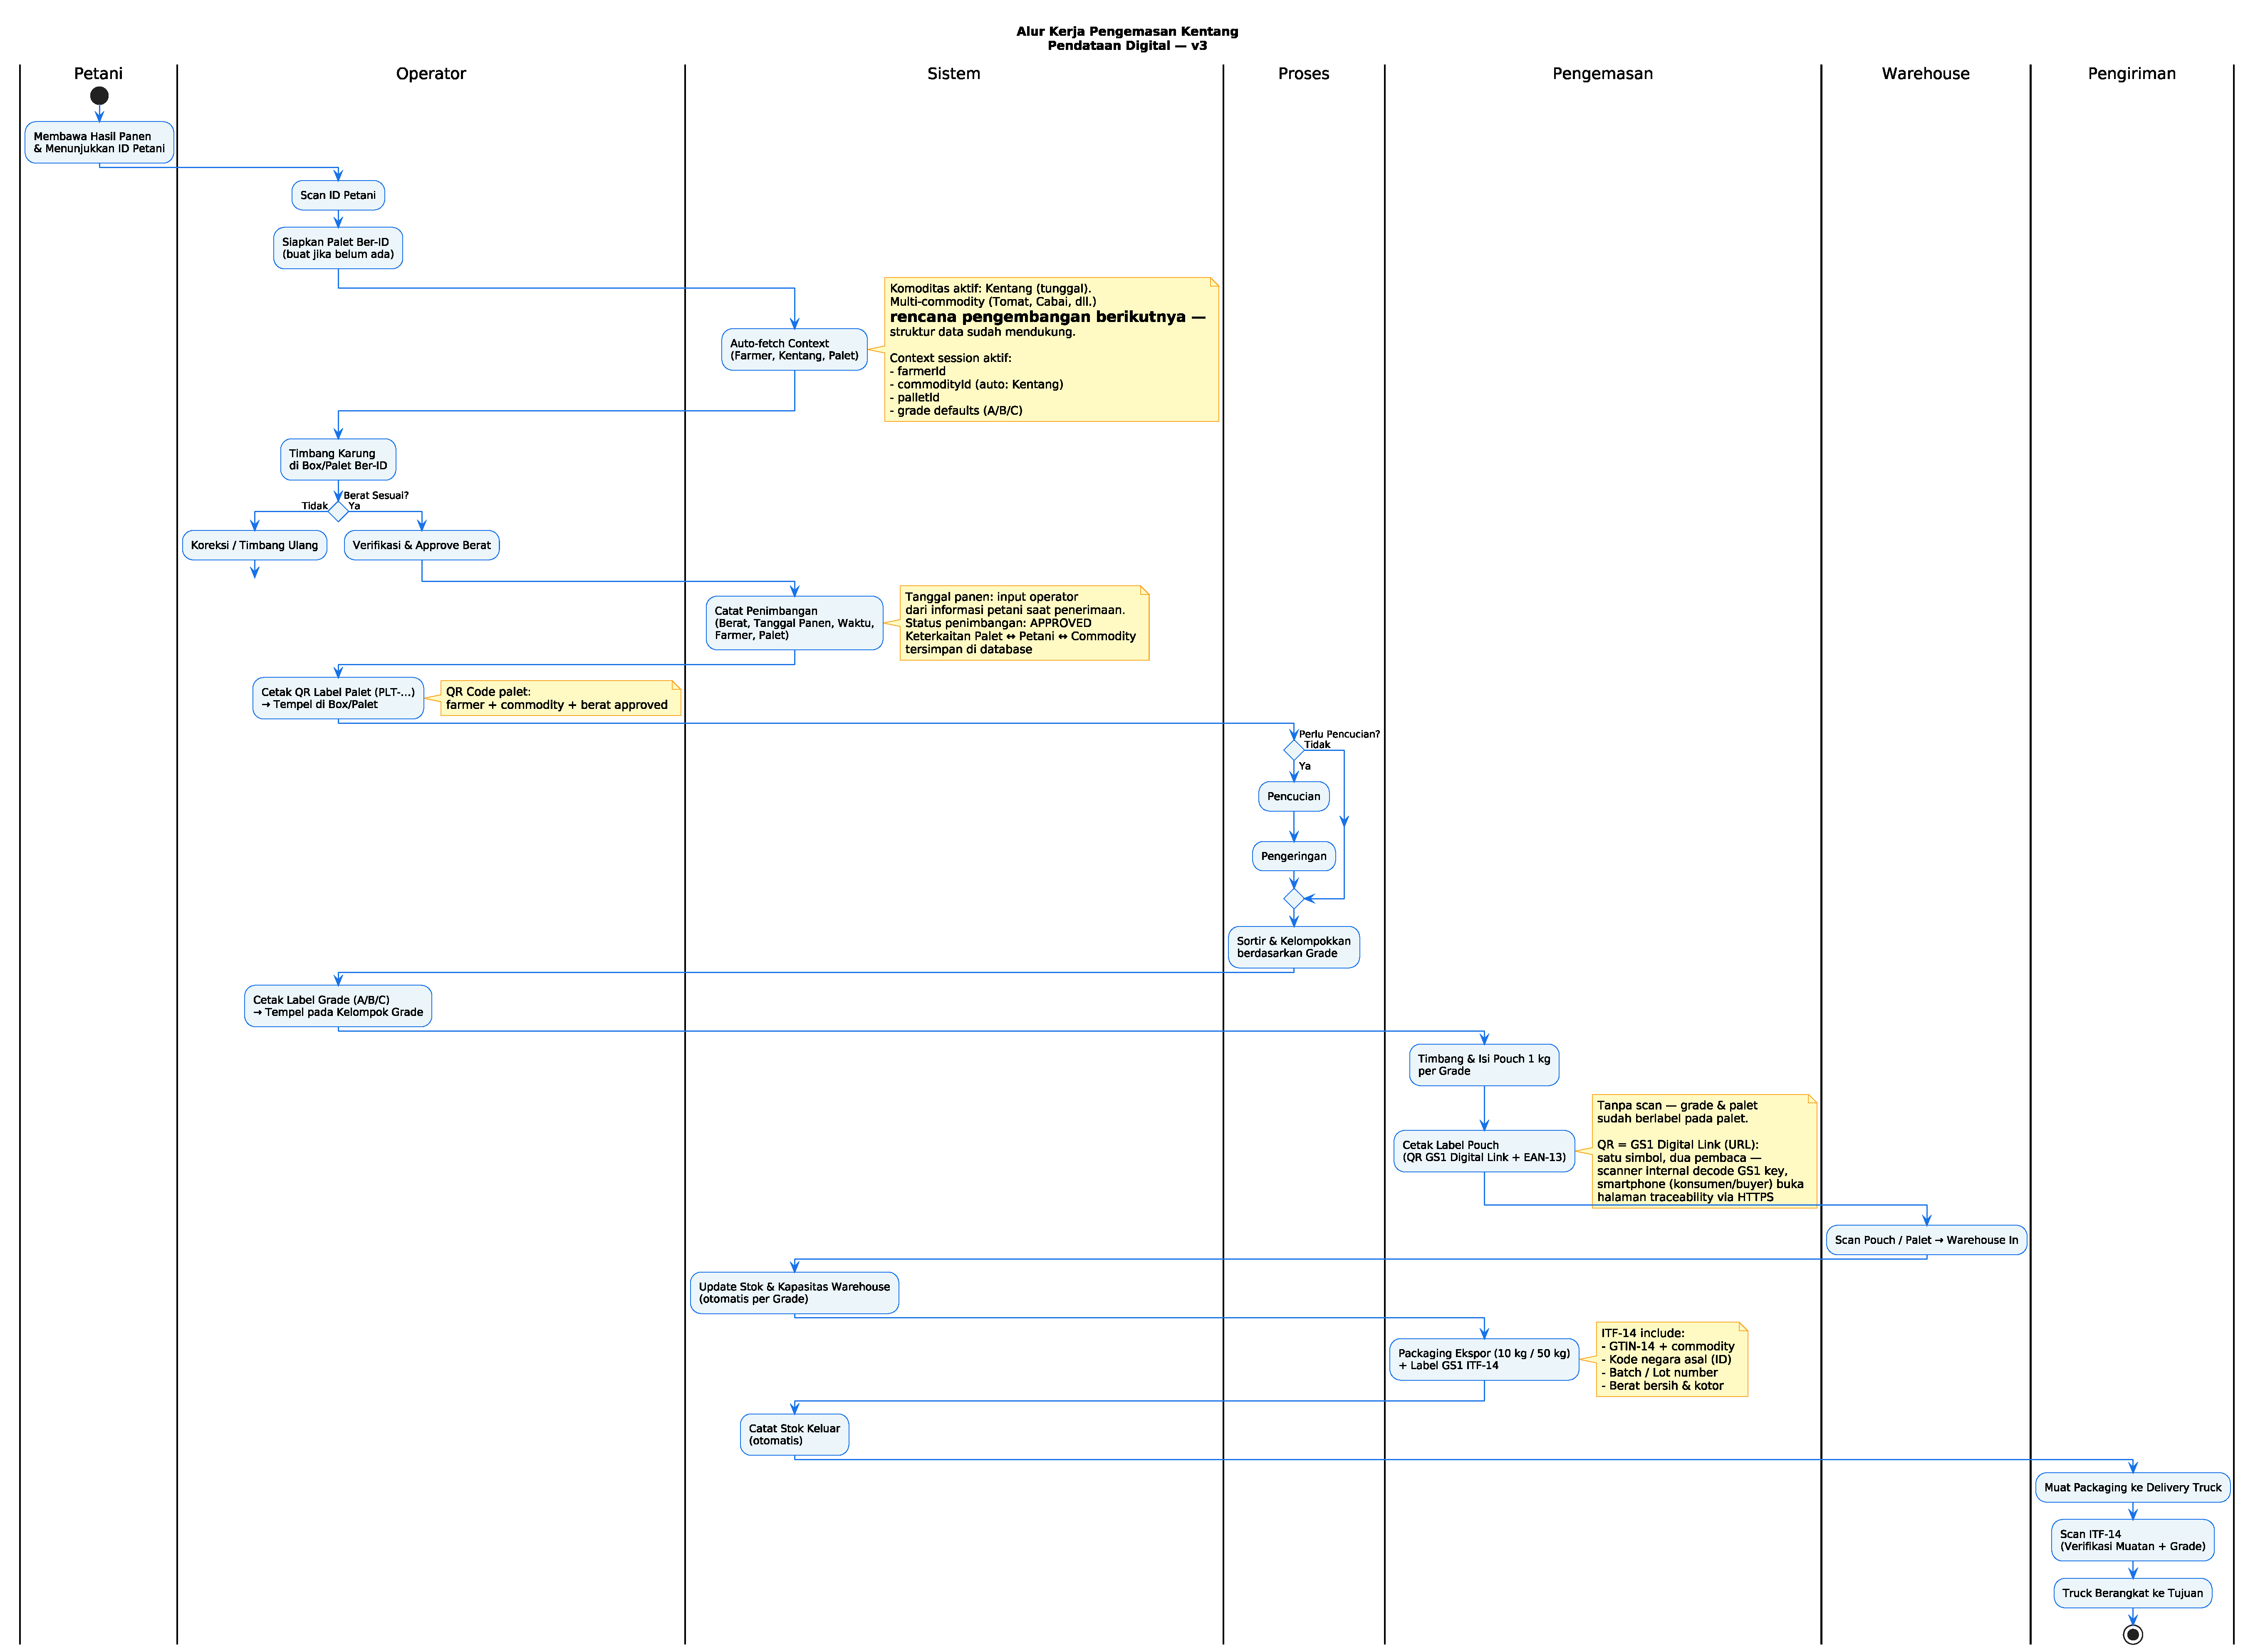
\includegraphics[width=\textwidth]{workflow}
  \caption{Diagram workflow pengemasan kentang (7 swimlane: Petani, Operator, Sistem,
  Proses, Pengemasan, Warehouse, Pengiriman).\newline
  (Sumber: \texttt{docs/DIAGRAM.md})}
\end{figure}

\subsection{Peran per Swimlane}
\begin{longtable}{@{}>{\raggedright\arraybackslash}p{2.6cm}>{\raggedright\arraybackslash}p{12.6cm}@{}}
\toprule
\textbf{Lane} & \textbf{Peran} \\
\midrule
\endhead
Petani & Membawa panen, menunjukkan ID petani, menyerahkan hasil panen \\
Operator & Scan ID, siapkan palet, timbang karung, verifikasi \& approve, cetak label palet; saat sortir: cetak label grade (A/B/C) \\
Sistem & Auto-fetch context, pencatatan otomatis (status \texttt{APPROVED}), update stok \& kapasitas, resolve GS1 Digital Link ke halaman traceability publik \\
Proses & Pencucian (opsional), sortir \& pengelompokan grade \\
Pengemasan & Timbang \& isi pouch 1 kg per grade, cetak label (QR GS1 Digital Link + EAN-13) --- tanpa scan, grade sudah terpisah di palet \\
Warehouse & Warehouse in (scan pouch/pallet), manajemen stok masuk/keluar \\
Pengiriman & Loading truck, verifikasi muatan + grade via ITF-14, keberangkatan \\
\bottomrule
\end{longtable}

% ============================================================================
\section{Standar Identifikasi \& Barcode}

Seluruh identifier mengikuti standar berikut (GS1 Indonesia):

\begin{longtable}{@{}>{\raggedright\arraybackslash}p{3.0cm}>{\raggedright\arraybackslash}p{6.6cm}>{\raggedright\arraybackslash}p{5.6cm}@{}}
\toprule
\textbf{Kode} & \textbf{Format} & \textbf{Penggunaan} \\
\midrule
\endhead
Farmer & \texttt{FRM-\{YYYY\}-\{SEQ\}} & QR pada ID card petani \\
Pallet & \texttt{PLT-\{YYYYMMDD\}-\{SEQ\}} & QR label palet, ditempel pada box/palet setelah approve \\
Grade & \texttt{GRD-\{PALLET\_CODE\}-\{GRADE\}} & Label grade pada kelompok hasil sortir di palet \\
Pouch QR & \texttt{https://\{domain\}/01/\{GTIN-13\}/}\newline\texttt{10/\{LOT\}/21/\{SERIAL\}} & QR GS1 Digital Link pada label pouch 1 kg \\
Pouch EAN-13 & \texttt{899\{COMMODITY\_CODE\}\{SEQ\}} & EAN-13 pada label pouch (\texttt{899} = kode negara Indonesia) \\
Packaging ITF-14 & \texttt{\{GTIN-14\}} & ITF-14 pada packaging ekspor 10 kg/50 kg \\
\bottomrule
\end{longtable}

\subsection{GS1 Digital Link pada Label Pouch}
Contoh konfigurasi URI pada QR label pouch:

{\scriptsize
\begin{verbatim}
https://trace.enyx.id/01/899001000001/10/PLT-20260914-0001-A/21/PCH-PLT-20260914-0001-001
                   |                |                    |
                 AI 01            AI 10                 AI 21
               (GTIN-13)      (batch/lot)            (serial)
\end{verbatim}
}

\begin{itemize}
  \item \textbf{Satu simbol, dua pembaca}: scanner internal mendecode element string GS1 (tanpa internet); smartphone (konsumen/buyer) mengikuti resolusi URL ke halaman traceability publik.
  \item Halaman traceability menampilkan: nama petani, lokasi kebun, tanggal panen, komoditas, grade, berat, serta status perjalanan produk.
  \item EAN-13 tetap dicetak paralel selama transisi 1D $\rightarrow$ 2D berlangsung.
  \item Resolver tersedia pada komponen \emph{Traceability Page + GS1 Digital Link Resolver} di Application Level; akses publik tanpa login.
\end{itemize}

\subsection{Ringkasan Barcode per Wadah}
\begin{longtable}{@{}>{\raggedright\arraybackslash}p{3.6cm}>{\raggedright\arraybackslash}p{3.4cm}>{\raggedright\arraybackslash}p{2.8cm}>{\raggedright\arraybackslash}p{5.2cm}@{}}
\toprule
\textbf{Wadah} & \textbf{Barcode} & \textbf{Standar} & \textbf{Fungsi} \\
\midrule
\endhead
Kelompok grade (palet) & QR/Barcode grade & Internal & Identifikasi grade (A/B/C) per kelompok sortir \\
Pouch 1 kg & QR GS1 Digital Link & GS1 internal + publik & Scanner internal decode GS1 key; smartphone konsumen buka halaman traceability \\
Pouch 1 kg & EAN-13 & GS1 ritel & Identifikasi produk ritel/ekspor \\
Packaging 10/50 kg & ITF-14 & GS1 logistik & Identifikasi kemasan logistik ekspor \\
\bottomrule
\end{longtable}

% ============================================================================
\section{Skema Data}

Skema database dirancang relasional (PostgreSQL) dengan perluasan TimescaleDB untuk
data time-series pembacaan sensor. Setiap tabel bisnis memiliki \texttt{commodityId}
sehingga multi-commodity cukup mengandalkan data master.

\begin{figure}[htbp]
  \centering
  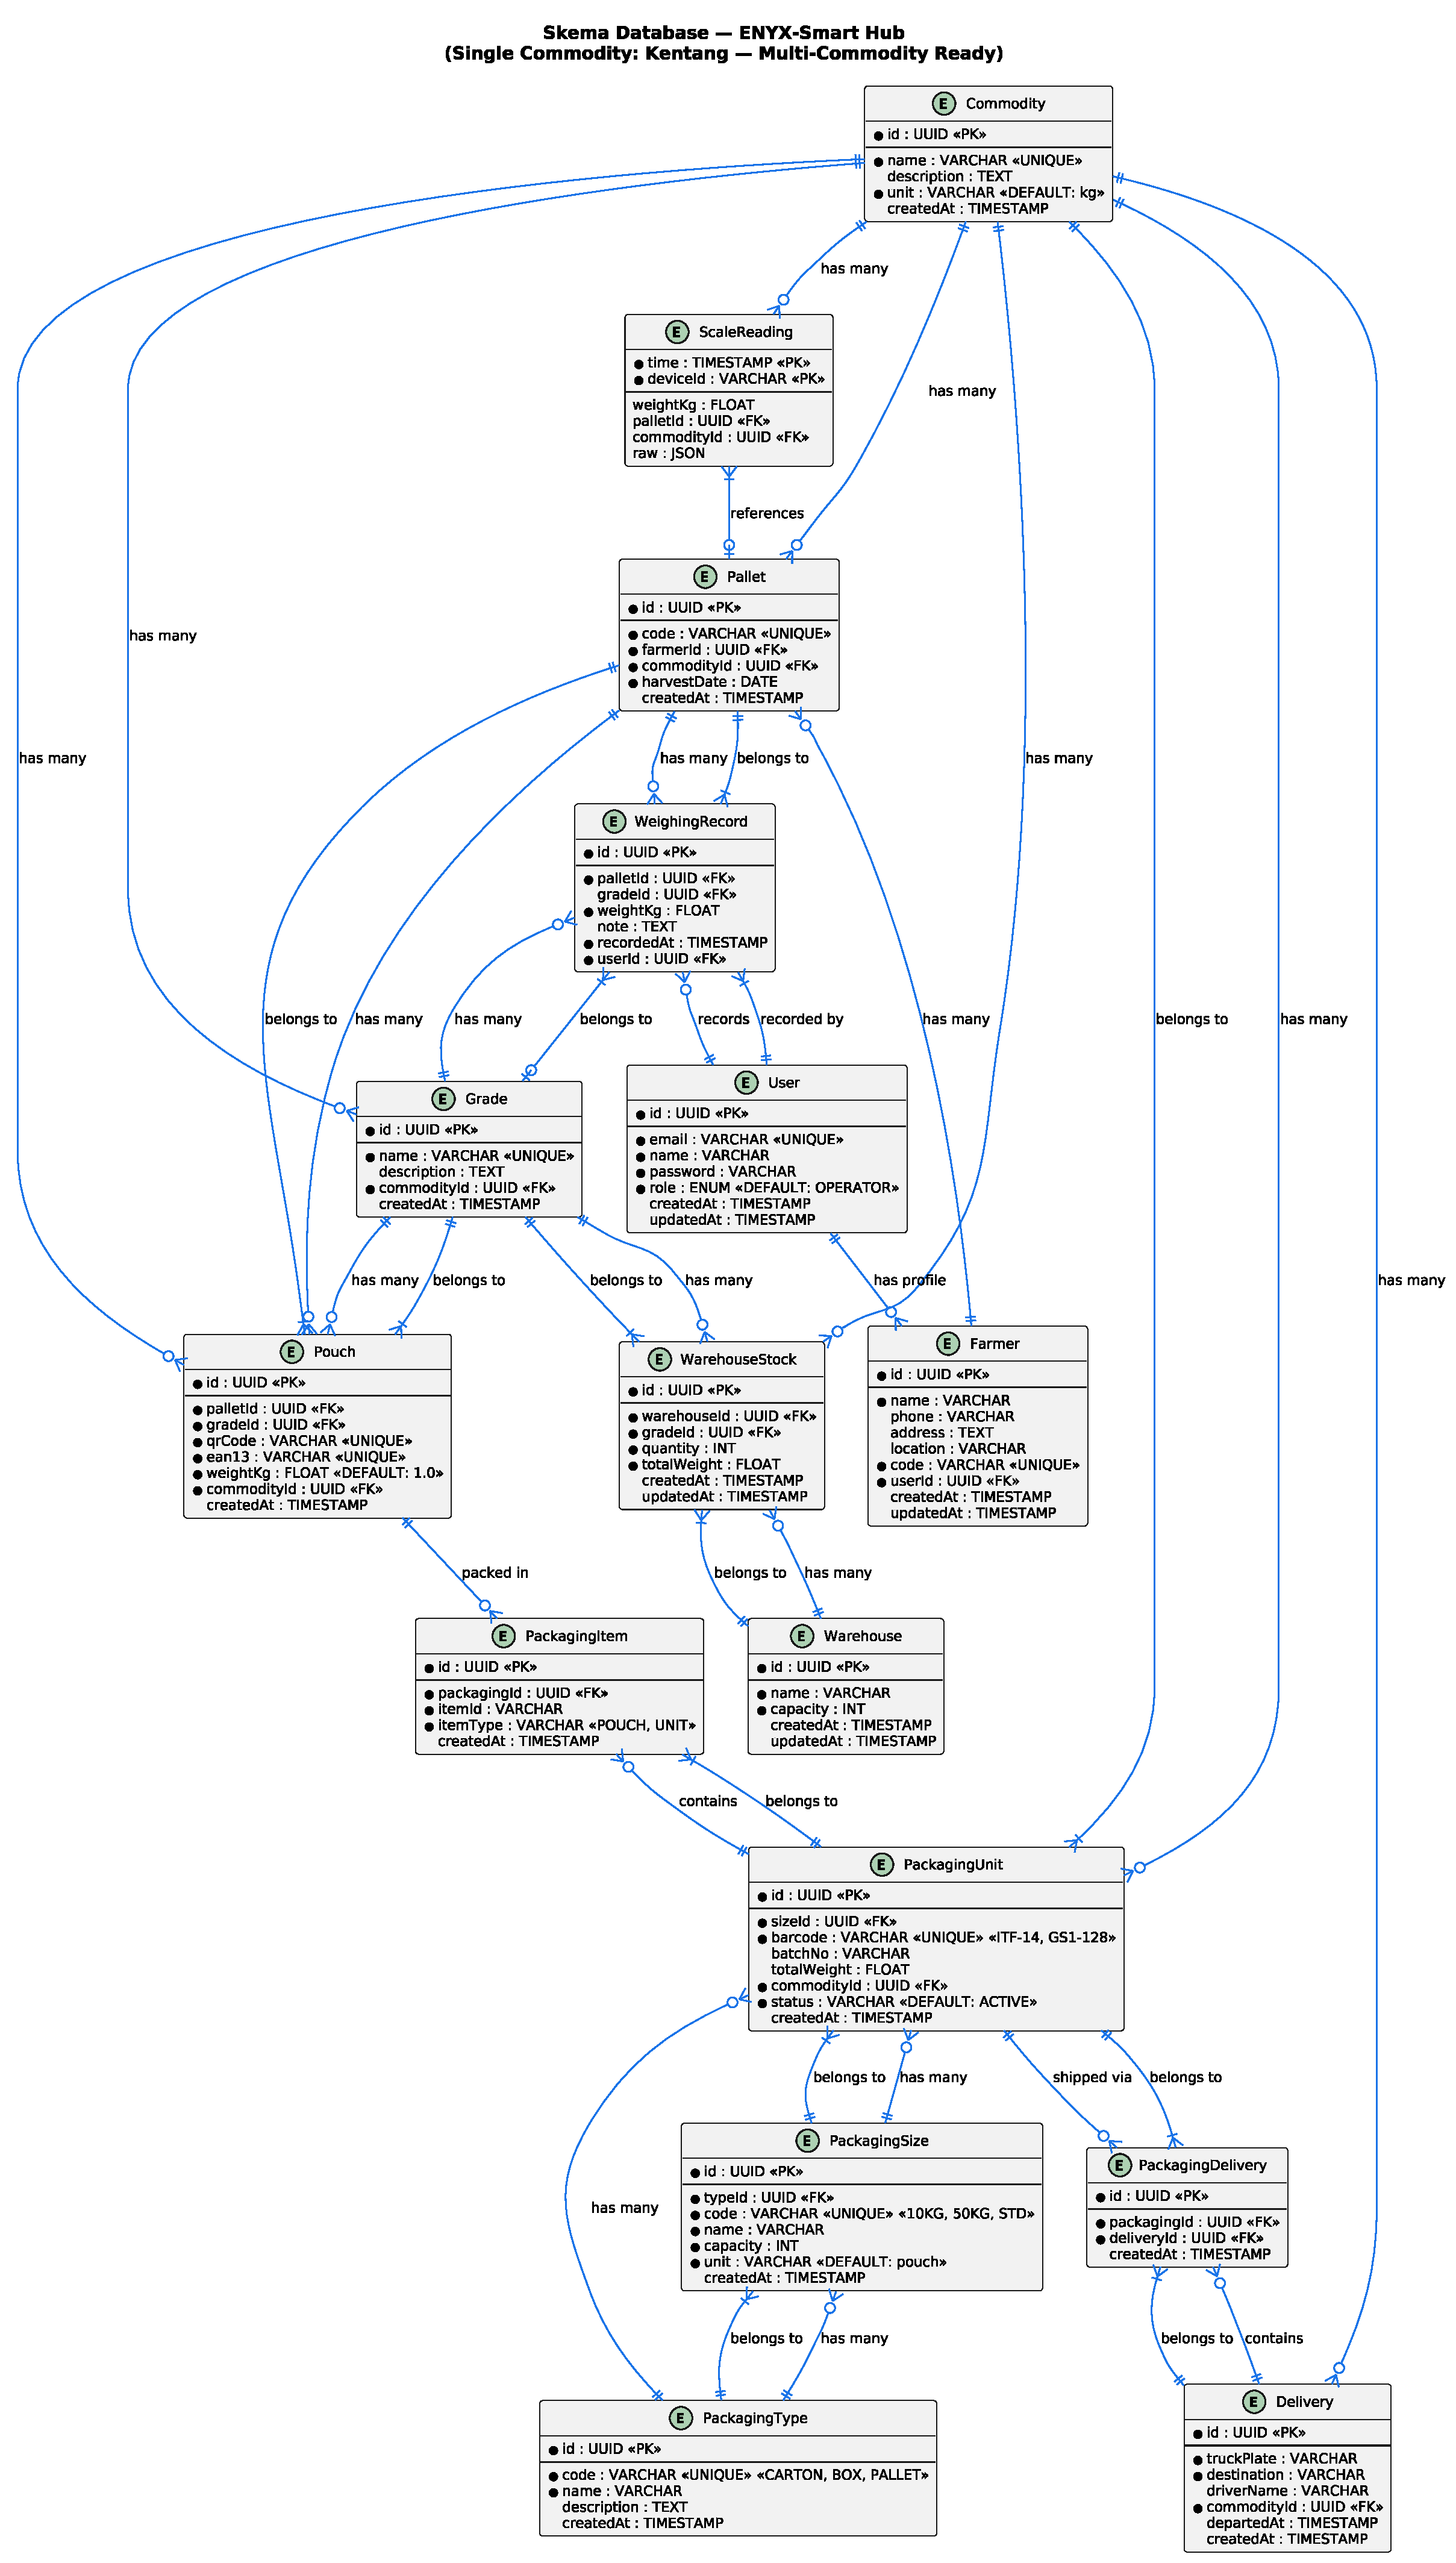
\includegraphics[width=0.72\textwidth]{database}
  \caption{Diagram skema database (ERD).\newline (Sumber: \texttt{docs/DIAGRAM.md})}
\end{figure}

\subsection{Entitas Inti}
\begin{longtable}{@{}>{\raggedright\arraybackslash}p{3.2cm}>{\raggedright\arraybackslash}p{11.0cm}@{}}
\toprule
\textbf{Entitas} & \textbf{Keterangan} \\
\midrule
\endhead
\texttt{commodity} & Master komoditas; saat ini hanya Kentang aktif (\texttt{001}); Tomat (\texttt{002}), Cabai (\texttt{003}) reserved \\
\texttt{grade} & Grade per komoditas (Kentang: A/B/C) \\
\texttt{farmer} / \texttt{user} & Data petani dan akun pengguna dengan role RBAC \\
\texttt{pallet} & Wadah/palet ber-ID kode \texttt{PLT}; memuat \texttt{farmerId}, \texttt{commodityId}, dan \texttt{harvestDate} (tanggal panen, input operator) \\
\texttt{weighing\_record} & Penimbangan per palet; status \texttt{APPROVED} oleh operator \\
\texttt{pouch} & Unit retail 1 kg; memuat kode \texttt{PCH}, QR GS1 Digital Link, dan EAN-13 \\
\texttt{warehouse\_stock} & Stok per grade; quantity dan total berat, tracking kapasitas \\
\texttt{packaging\_*} & Tipe, ukuran, unit packaging (10/50 kg), dan relasi item--packaging \\
\texttt{delivery} & Pengiriman: truck, tujuan, verifikasi ITF-14, keberangkatan \\
\texttt{scale\_reading} & Time-series (hypertable) pembacaan timbangan dari MQTT \\
\bottomrule
\end{longtable}

% ============================================================================
\section{Tech Stack}

\begin{longtable}{@{}>{\raggedright\arraybackslash}p{3.2cm}>{\raggedright\arraybackslash}p{4.6cm}>{\raggedright\arraybackslash}p{7.2cm}@{}}
\toprule
\textbf{Layer} & \textbf{Teknologi} & \textbf{Alasan} \\
\midrule
\endhead
Edge/MCU & ESP32 + PlatformIO & WiFi + MQTT native, RS485 via modul MAX485, hemat biaya \\
MQTT Broker & Eclipse Mosquitto 2.x & Ringan, stabil untuk LAN, QoS 0/1/2, autentikasi perangkat \\
Backend & Node.js 20 + Express 5 + TypeScript & Ekosistem MQTT matang, real-time mudah, type safety \\
ORM & Prisma & Query type-safe, migrasi terkelola \\
Database & PostgreSQL 17 + TimescaleDB & Relasional untuk bisnis + time-series IoT dalam satu server \\
Frontend & React 19 + TypeScript + Vite & Modern, HMR cepat, ekosistem luas \\
Styling & Tailwind CSS v4 (komponen kustom) & Konsisten, cepat dikembangkan; shadcn/ui opsional roadmap \\
Real-time & Socket.io 4 \textit{(rencana)} & WebSocket + fallback otomatis untuk dashboard live; belum terpasang di frontend \\
Auth & JWT + RBAC middleware & Stateless, sesuai skema role operasional \\
Barcode & bwip-js + html5-qrcode \textit{(rencana)} & Untuk generate/scan EAN-13, ITF-14, QR/GS1 Digital Link; belum terpasang \\
Cloud/Backup & Neon/Supabase PostgreSQL & Managed PITR tanpa ribet \\
Infra & Docker Compose + Nginx + Let's Encrypt & Deploy di satu PC server, HTTPS siap \\
\bottomrule
\end{longtable}

Struktur repositori mengikuti pemisahan \texttt{firmware/} (sketsa ESP32),
\texttt{backend/} (modular monolith + Prisma), dan \texttt{frontend/} (React SPA),
dengan Docker Compose sebagai orkestrasi lokal.

% ============================================================================
\section{Perangkat Keras (BOM Ringkas)}

Estimasi biaya perangkat keras dan infrastruktur berdasarkan harga pasar Indonesia
(September 2026). Sumber: e-commerce dan distributor lokal (Shopee, Tokopedia,
Blueprint Indonesia, Indotrading, PT. Altraman).

\begin{longtable}{@{}>{\raggedright\arraybackslash}p{5.4cm}>{\raggedright\arraybackslash}p{2.6cm}>{\raggedright\arraybackslash}p{2.6cm}>{\raggedright\arraybackslash}p{2.6cm}@{}}
\toprule
\textbf{Kategori} & \textbf{Minimum} & \textbf{Maksimum} & \textbf{Rekomendasi} \\
\midrule
\endhead
Edge / MCU \& IoT & Rp 2.390.000 & Rp 3.500.000 & Rp 2.900.000 \\
Field Devices & Rp 14.500.000 & Rp 24.000.000 & Rp 18.000.000 \\
Networking \& Infrastruktur & Rp 4.500.000 & Rp 7.500.000 & Rp 5.500.000 \\
Application Server \& Database & Rp 12.750.000 & Rp 18.000.000 & Rp 14.500.000 \\
Consumables \& Spare Parts & Rp 920.000 & Rp 1.500.000 & Rp 1.200.000 \\
Testing \& Kalibrasi & Rp 1.950.000 & Rp 2.500.000 & Rp 2.000.000 \\
Safety \& Protection & Rp 760.000 & Rp 1.200.000 & Rp 900.000 \\
Software Licenses \& Services (1 tahun) & Rp 575.000 & Rp 4.000.000 & Rp 2.000.000 \\
\midrule
\textbf{TOTAL} & \textbf{Rp 38.345.000} & \textbf{Rp 62.200.000} & \textbf{Rp 47.000.000} \\
\bottomrule
\end{longtable}

\textbf{Catatan penting:}
\begin{itemize}
  \item Penyesuaian terkait aturan penimbangan baru: timbangan 100 kg RS485 hanya diperlukan untuk \emph{dua lokasi} (Area Penerimaan dan Area Pengemasan), bukan tiga stasiun grade. Detail komponen tetap mengacu pada struktur BOM; revisi qty/price adalah langkah procurement berikutnya.
  \item Timbangan sebaiknya dibeli dari distributor resmi (PT. Altraman, Rice Lake) untuk garansi dan kalibrasi.
  \item Software inti semuanya open source (lisensi Rp 0); biaya layanan opsional adalah cloud backup, domain, dan SSL gratis.
\end{itemize}

% ============================================================================
\section{UI/UX}

\subsection{Prinsip Desain}
Minimalis (tanpa shadow/dekorasi berlebih), konsisten antar-role, fungsional,
mobile-first responsif, dan aksesibel (kontras tinggi, font readable).

\subsection*{Status Implementasi Frontend}
Frontend berjalan sebagai SPA React 19 + Vite + Tailwind v4 (\texttt{npm run dev},
port 5173, proxy \texttt{/api} ke backend). Saat ini memakai komponen kustom dan
mock data lokal; halaman traceability konsumen telah terpasang sebagai route
publik \texttt{/traceability}. Dialog konfirmasi, toast, integrasi kamera
(\texttt{html5-qrcode}), koneksi backend/WebSocket, dan mode input timbangan
Auto (Modbus TCP) / Manual menjadi pekerjaan berikutnya mengikuti spesifikasi di
section ini.

\subsection{Palet Warna \& Tipografi}
Palet berikut adalah design system yang **terpasang di frontend** (Tailwind v4
\texttt{@theme} pada \texttt{frontend/src/styles/index.css}):

\begin{longtable}{@{}>{\raggedright\arraybackslash}p{3.4cm}>{\raggedright\arraybackslash}p{2.6cm}>{\raggedright\arraybackslash}p{9.0cm}@{}}
\toprule
\textbf{Warna} & \textbf{Hex} & \textbf{Penggunaan} \\
\midrule
\endhead
Primary & \texttt{\#000000} & Tombol utama, link aktif, heading \\
Primary Hover & \texttt{\#333333} & Hover state tombol utama \\
Accent & \texttt{\#0070f3} & Aksen, spinner, tanda aktif pada journey \\
Accent Hover & \texttt{\#0051a8} & Hover state aksen \\
Danger & \texttt{\#e00} / \texttt{\#c00} & Aksi berisiko, tombol logout \\
Background & \texttt{\#fafafa} & Background page dan sidebar \\
Surface & \texttt{\#ffffff} & Background card dan navbar \\
Text & \texttt{\#171717} / \texttt{\#666666} / \texttt{\#999999} & Teks utama, sekunder, redup \\
Border & \texttt{\#eaeaea} & Border, divider, tabel \\
\bottomrule
\end{longtable}

Tipografi: \textbf{Inter} (weight 400--700, di-load dari Google Fonts), base
16px, line-height 1.5; font monospace untuk blok kode dan nomor seri.

\subsection{Layar per Role}
\begin{longtable}{@{}>{\raggedright\arraybackslash}p{3.4cm}>{\raggedright\arraybackslash}p{11.6cm}@{}}
\toprule
\textbf{Role} & \textbf{Fokus layar} \\
\midrule
\endhead
Admin & Manajemen pengguna dan komoditas, laporan, konfigurasi sistem \\
Weighing Operator & Input cepat: scan ID, timbang, approve; metrik weighing hari ini dan palet aktif \\
Sorting Operator & Sortir grade, cetak label grade, konfirmasi hasil sortir (tanpa timbang) \\
Packing Operator & Timbang \& isi pouch, preview \& cetak label (QR + EAN-13) \\
Warehouse Operator & Scan warehouse in/out, ringkasan stok per grade, alert kapasitas \\
Delivery Operator & Loading truck, scan ITF-14 verifikasi muatan, catat keberangkatan \\
Farmer & Riwayat setoran dan traceability gaya mobile-banking: total pengiriman, aktivitas terbaru, pencarian barcode \\
Konsumen (publik) & Halaman traceability hasil scan QR GS1 Digital Link, tanpa login \\
\bottomrule
\end{longtable}

\subsection{Hierarki Halaman}

Struktur halaman disusun mengikuti alur kerja dan role. Spesifikasi berikut
mencakup **fungsi dan tujuan tiap halaman** (bukan detail layout visual).

{\scriptsize
\begin{verbatim}
ENYX-Smart Hub
+-- Publik (tanpa login)
|   +-- Traceability Konsumen        — publik, /traceability: input/scan kode PCH-/PLT-
+-- Autentikasi
|   +-- Login                        — masuk semua role internal
+-- Admin
|   +-- Dashboard                    — ringkasan operasional sistem
|   +-- Manajemen Pengguna           — akun & role (Weighing/Sorting/Packing/Warehouse/Delivery/Farmer)
|   +-- Master Data                  — petani, grade (A/B/C), perangkat (timbangan, printer, scanner)
|   +-- Laporan & Analitik           — rekap setoran, stok, pengiriman
|   +-- Pengaturan Sistem            — komoditas aktif (Kentang), parameter timbangan, konfigurasi label
+-- Weighing Operator (Area Penerimaan)
|   +-- Scan & Context               — scan ID petani; buat/siapkan palet ber-ID
|   +-- Penimbangan Karung           — input berat, koreksi bila perlu, approve
|   +-- Cetak Label Palet            — preview & cetak QR label PLT-...
|   +-- Riwayat Timbang              — daftar setoran yang sudah di-approve
+-- Sorting Operator (Area Sortir)
|   +-- Sortir Grade                 — kelompokkan hasil panen ke grade A/B/C
|   +-- Cetak Label Grade            — cetak & tempel label GRD-... per kelompok
|   +-- Riwayat Sortir               — rekap hasil sortir per palet
+-- Packing Operator (Area Pengepakan)
|   +-- Timbang & Isi Pouch 1 kg     — timbang pouch per grade (tanpa scan)
|   +-- Cetak Label Pouch            — preview & cetak QR GS1 Digital Link + EAN-13
|   +-- Riwayat Pengemasan           — daftar pouch yang sudah berlabel
+-- Warehouse Operator
|   +-- Warehouse In                 — scan pouch/pallet, catat stok masuk
|   +-- Warehouse Out                — packaging ekspor 10/50 kg + label ITF-14
|   +-- Status Stok & Kapasitas      — stok per grade, sisa kapasitas
|   +-- Alert Kapasitas              — notifikasi kapasitas menipis/penuh
+-- Delivery Operator
|   +-- Buat Delivery                — susun muatan dari packaging unit
|   +-- Verifikasi Muatan            — scan ITF-14 (jumlah, grade, batch, tujuan)
|   +-- Keberangkatan                — catat truck, tujuan, waktu berangkat
+-- Petani
    +-- Beranda                      — ringkasan setoran & aktivitas terbaru
    +-- Setoran Saya                 — riwayat setoran per palet/grade
    +-- My QR (/dashboard/traceability) — QR identitas petani untuk discan operator
    +-- Lacak Produk (/traceability)   — halaman traceability publik (tanpa login)
    +-- Profil                       — data petani & lokasi kebun
\end{verbatim}
}

\begin{longtable}{@{}>{\raggedright\arraybackslash}p{3.0cm}>{\raggedright\arraybackslash}p{3.6cm}>{\raggedright\arraybackslash}p{4.2cm}>{\raggedright\arraybackslash}p{4.2cm}@{}}
\toprule
\textbf{Grup} & \textbf{Halaman} & \textbf{Fungsi} & \textbf{Tujuan} \\
\midrule
\endhead
Publik & Traceability Konsumen & Menampilkan data asal-usul produk (petani, kebun, tanggal panen, grade, berat, perjalanan) dari kode QR yang di-scan/dimasukkan; terpasang di route \texttt{/traceability} (entri dari landing page), data masih contoh sampai backend aktif & Memberi transparansi kepada konsumen/buyer tanpa perlu akun \\
\hline
Weighing Operator & Scan \& Context & Scan ID petani, buat palet ber-ID, aktivasi session context & Memastikan setiap setoran terhubung ke petani dan palet yang benar sejak awal \\
\hline
Weighing Operator & Penimbangan Karung & Input berat + tanggal panen, tombol Approve dan Koreksi/Timbang Ulang, status \texttt{PENDING}/\texttt{APPROVED} per record & Menetapkan berat setoran resmi sebagai data awal \\
\hline
Weighing Operator & Cetak Label Palet & Preview dan cetak QR label \texttt{PLT-...} & Memberi identitas fisik palet yang dapat di-scan di tahap berikutnya \\
\hline
Sorting Operator & Sortir \& Label Grade & Kelompokkan grade A/B/C, cetak \& tempel label grade per kelompok & Memisahkan mutu dan memberi penanda grade pada palet \\
\hline
Packing Operator & Timbang \& Isi Pouch & Timbang dan isi pouch 1 kg per grade tanpa scan & Menghasilkan unit retail dengan berat akurat \\
\hline
Packing Operator & Cetak Label Pouch & Preview dan cetak label QR GS1 Digital Link + EAN-13 & Memberi identitas GS1 dan kanal traceability pada tiap pouch \\
\hline
Warehouse Operator & Warehouse In/Out & Scan pouch/pallet untuk stok masuk; scan packaging untuk stok keluar & Menjaga stok terdata dan kapasitas terkendali \\
\hline
Warehouse Operator & Status Stok \& Kapasitas & Ringkasan stok per grade dan sisa kapasitas & Mendukung keputusan penyimpanan dan pengambilan stok \\
\hline
Delivery Operator & Verifikasi Muatan & Scan ITF-14 untuk mencocokkan jumlah, grade, batch, dan tujuan & Mencegah salah kirim sebelum truck berangkat \\
\hline
Petani & Setoran Saya \& My QR & Riwayat setoran per palet/grade; QR identitas petani untuk discan operator & Memberi visibilitas hasil panen dan memperkuat kepercayaan \\
\bottomrule
\end{longtable}

\subsection{Spesifikasi Responsivitas Mobile}

Operator bekerja dengan tablet atau smartphone di stasiun kerja, sehingga seluruh
halaman dirancang \emph{mobile-first} dan berfungsi penuh pada layar kecil.

\begin{longtable}{@{}>{\raggedright\arraybackslash}p{3.2cm}>{\raggedright\arraybackslash}p{5.6cm}>{\raggedright\arraybackslash}p{6.2cm}@{}}
\toprule
\textbf{Aspek} & \textbf{Spesifikasi} & \textbf{Alasan} \\
\midrule
\endhead
Breakpoint & Mobile $<$ 768px; Tablet 768--1024px; Desktop $\geq$ 1024px & Satu kode base untuk tablet stasiun dan desktop admin \\
\hline
Navigasi & Navbar menyusut menjadi menu ringkas (hamburger) di bawah 768px; area konten memenuhi lebar layar dengan padding 16px & Layar sempit di stasiun harus tetap terjangkau satu tangan \\
\hline
Target sentuh & Tombol aksi utama minimum 44$\times$44px; aksi kritis (Simpan, Approve, Cetak) ditempatkan tetap (sticky) di bagian bawah & Operator bersarung tangan dan bekerja cepat; mencegah salah tekan \\
\hline
Tabel data & Pada mobile, baris tabel berubah menjadi daftar kartu atau tabel dengan scroll horizontal; maksimal 3 kolom prioritas ditampilkan & Tabel lebar tidak terbaca di layar $<$ 768px \\
\hline
Input berat & Field numerik memakai keypad numerik besar; pada mode Auto pembacaan Modbus TCP tampil real-time dan terkunci ke field berat saat stabil & Meminimalkan typing saat menimbang \\
\hline
Scan barcode & Pemindaian memakai kamera perangkat (target: \texttt{html5-qrcode}) dengan area fokus besar; fallback input manual kode & Scanner USB tetap didukung di desktop \\
\hline
Orientasi & Halaman penimbangan dan pengepakan mendukung orientasi landscape dengan tampilan angka besar & Posisi timbangan sering memaksa perangkat miring \\
\hline
PWA \& offline & Halaman aktif dapat di-cache; data context disimpan lokal; aksi scan/input masuk antrean saat offline dan dikirim saat koneksi kembali & Internet fasilitas sesekali terputus \\
\hline
Tipografi & Font minimum 16px pada input (mencegah auto-zoom iOS) & Kenyamanan membaca dan mengisi di lapangan \\
\hline
Aksesibilitas & Kontras warna memenuhi rasio AA; seluruh aksi dapat dijangkau tanpa hover (khususnya tombol cetak dan approve) & Digunakan di lingkungan tidak selalu ideal \\
\hline
Performa & Halaman di luar halaman aktif dimuat lazy; preview label dioptimalkan (render terjadwal) & Perangkat kelas menengah tetap responsif \\
\bottomrule
\end{longtable}

\subsection{RBAC}
Role diimplementasikan sebagai klaim \texttt{role} pada JWT dengan middleware
verifikasi di setiap endpoint: \texttt{ADMIN}, \texttt{WEIGHING\_OPERATOR},
\texttt{SORTING\_OPERATOR}, \texttt{WAREHOUSE\_OPERATOR},
\texttt{DELIVERY\_OPERATOR}, \texttt{FARMER}. Konsumen mengakses halaman
traceability publik tanpa autentikasi.

\subsection{Input Timbangan: Auto (Modbus TCP) \& Manual}

Timbangan terhubung melalui \textbf{Modbus TCP} (backend sebagai Modbus client
membaca holding register timbangan melalui jaringan LAN). Operator memilih dua
mode input pada setiap form penimbangan:

\begin{longtable}{@{}>{\raggedright\arraybackslash}p{2.6cm}>{\raggedright\arraybackslash}p{6.2cm}>{\raggedright\arraybackslash}p{6.2cm}@{}}
\toprule
\textbf{Aspek} & \textbf{Mode Auto} & \textbf{Mode Manual} \\
\midrule
\endhead
Cara pakai & Operator menekan tombol \textbf{Auto}; sistem langsung membaca berat dari timbangan via Modbus TCP & Operator mengetik berat yang terlihat pada indikator timbangan \\
\hline
Tampilan & Angka berat besar (live, refresh $\pm$200--500ms) dengan tanda \emph{live}; nilai terkunci setelah stabil & Field input angka biasa dengan keypad numerik \\
\hline
Stabilitas & Indikator ``stabil'' saat perubahan berat $<$ ambang (misal $\pm$20g) selama $\pm$2 detik; tombol \textbf{Gunakan Nilai Ini} aktif saat stabil & Tidak ada; operator memastikan sendiri \\
\hline
Status koneksi & Menampilkan alamat timbangan (IP:port), status \emph{connected/disconnected}, waktu pembacaan terakhir & Tidak bergantung koneksi \\
\hline
Kegagalan & Timeout/tidak terjangkau muncul notifikasi + saran lanjut manual; nilai live ditandai jelas berbeda dari nilai manual & Selalu tersedia sebagai fallback \\
\hline
Berlaku di & Area Penerimaan (timbang karung) dan Area Pengepakan (timbang pouch 1 kg) & Sama \\
\bottomrule
\end{longtable}

\textbf{Perilaku tambahan:}
\begin{itemize}
  \item Mode disimpan per stasiun selama sesi operator; stasiun dengan timbangan terhubung default \emph{Auto}.
  \item Pada pengepakan pouch, mode Auto menampilkan target \textbf{1 kg} dengan toleransi (misal $\pm$5g) dan indikator ``muat sampai target''.
  \item Validasi berat: harus $>$ 0 dan tidak melebihi kapasitas timbangan; nilai di-lock ke field sebelum record dibuat (status \texttt{PENDING} menunggu approve).
  \item Backend bertugas melakukan polling Modbus TCP, timeout, dan penskalaan nilai sesuai resolusi timbangan (misal 5g/10g) --- aspek tersebut di luar lingkup UI/UX ini.
\end{itemize}

Catatan: integrasi Modbus TCP pada backend dan antarmuka Auto/Manual pada
frontend merupakan pekerjaan implementasi berikutnya; spesifikasi di atas menjadi
acuan desain interaksinya.

\subsection{Session Context Indicator}

Session context adalah elemen UI paling kritis bagi operator: salah petani atau
salah palet berarti data penimbangan tercatat ke entitas yang salah. Spesifikasi
berikut memastikan operator selalu sadar konteks aktif.

\begin{longtable}{@{}>{\raggedright\arraybackslash}p{3.2cm}>{\raggedright\arraybackslash}p{4.6cm}>{\raggedright\arraybackslash}p{7.4cm}@{}}
\toprule
\textbf{Elemen} & \textbf{Tampilan} & \textbf{Perilaku} \\
\midrule
\endhead
Context bar & Sticky di bagian atas semua halaman operator (di bawah navbar); latar
  \texttt{\#EAF4FB} (enyxlight) & Selalu terlihat; tidak bisa di-scroll hilang;
  muncul setelah scan pertama berhasil \\
\hline
Informasi yang ditampilkan & \textbf{Nama Petani} | \textbf{Kode Palet} |
  \textbf{Grade Default} & Diambil dari session context Redis; diperbarui via
  event \texttt{context:updated} (Socket.io) \\
\hline
Tombol Reset Context & Teks merah (\texttt{Reset}), ikon sampah, pojok kanan
  context bar & Memunculkan dialog konfirmasi destruktif sebelum reset;
  setelah reset, context bar hilang hingga scan berikutnya \\
\hline
Timeout indicator & Progress bar tipis (2px) di bawah context bar; memudar
  saat TTL Redis mendekati habis (TTL 4 jam) & Memberi peringatan visual
  sebelum sesi habis; operator dapat memperpanjang dengan aktivitas apapun \\
\hline
Status offline & Context bar berubah warna menjadi abu-abu dengan ikon
  peringatan bila koneksi WebSocket terputus & Operator tahu data mungkin
  belum tersinkron \\
\bottomrule
\end{longtable}

\subsection{Feedback Visual \& State Indikator}

Setiap aksi kritis harus memberikan umpan balik langsung agar operator tidak
bertanya-tanya apakah aksi sudah berhasil atau gagal.

\begin{longtable}{@{}>{\raggedright\arraybackslash}p{3.4cm}>{\raggedright\arraybackslash}p{3.8cm}>{\raggedright\arraybackslash}p{7.6cm}@{}}
\toprule
\textbf{Sumber} & \textbf{Indikator} & \textbf{Spesifikasi} \\
\midrule
\endhead
Koneksi MQTT / timbangan & Badge status di navbar & Hijau (\texttt{Connected})
  / Abu-abu (\texttt{Disconnected}) / Kuning (\texttt{Reconnecting}); diperbarui
  real-time via event \texttt{scale:status} \\
\hline
Pembacaan timbangan live & Field berat real-time & Angka diperbarui langsung
  dari event \texttt{scale:reading}; background field berkedip hijau saat
  nilai stabil ($\pm$0,05~kg selama 1~detik) \\
\hline
Approve berat & Toast sukses + suara klik & Toast hijau muncul 3~detik;
  status \texttt{APPROVED} terupdate di tabel riwayat tanpa refresh halaman \\
\hline
Cetak label & Toast + indikator antrean cetak & Toast kuning \emph{Printing\ldots}
  saat perintah dikirim; berubah hijau jika berhasil atau merah jika timeout
  (10~detik) \\
\hline
Scan barcode berhasil & Animasi border hijau + suara beep & Area kamera
  mendapat border hijau 500~ms; data petani/palet langsung populate ke form \\
\hline
Scan barcode gagal & Border merah + pesan inline & Pesan \emph{``Barcode not
  recognized --- try manual input''} muncul di bawah area scan \\
\hline
Koneksi WebSocket & Banner kuning sticky di atas context bar & Muncul saat
  WebSocket terputus: \emph{``Real-time connection lost. Data may be delayed.''}
  Hilang otomatis saat reconnect \\
\hline
Aksi loading & Skeleton screen + spinner pada tombol & Tombol aksi menampilkan
  spinner dan menjadi \texttt{disabled} selama request berlangsung; mencegah
  double-submit \\
\bottomrule
\end{longtable}

\subsection{Skala Tipografi}

Selain basis font Poppins 16px yang sudah ditetapkan, skala berikut mengatur
hierarki visual secara konsisten di seluruh halaman:

\begin{longtable}{@{}>{\raggedright\arraybackslash}p{3.0cm}>{\raggedright\arraybackslash}p{2.2cm}>{\raggedright\arraybackslash}p{2.0cm}>{\raggedright\arraybackslash}p{7.8cm}@{}}
\toprule
\textbf{Token} & \textbf{Ukuran} & \textbf{Weight} & \textbf{Penggunaan} \\
\midrule
\endhead
\texttt{display} & 32px & 700 & Angka berat real-time, total stok --- elemen
  yang harus terbaca dari jarak jauh \\
\hline
\texttt{h1} & 24px & 700 & Judul halaman (satu per halaman) \\
\hline
\texttt{h2} & 20px & 600 & Sub-judul bagian, judul kartu \\
\hline
\texttt{h3} & 18px & 600 & Label grup form, judul kolom tabel \\
\hline
\texttt{body} & 16px & 400 & Teks utama, isi tabel, label input \\
\hline
\texttt{body-medium} & 16px & 500 & Nilai penting dalam tabel (berat, kode palet) \\
\hline
\texttt{small} & 14px & 400 & Teks sekunder, placeholder, caption tabel \\
\hline
\texttt{caption} & 12px & 400 & Timestamp, keterangan gambar, label badge \\
\bottomrule
\end{longtable}

\textbf{Aturan tambahan:} Tidak ada teks di bawah 12px pada antarmuka operasional.
Input numerik (berat, jumlah pouch) menggunakan token \texttt{display} agar terbaca
dari jarak wajar stasiun kerja. Seluruh teks pada input field minimal 16px untuk
mencegah auto-zoom pada browser iOS.

\subsection{Komponen Antarmuka (Terpasang \& Target)}

Komponen kritis saat ini diimplementasikan sebagai \textbf{komponen kustom +
Tailwind v4} pada \texttt{frontend/src} (Card, DataTable, Logo, PlaceholderPage,
badge, tabel, spinner, alert-box di \texttt{styles/index.css}). Migrasi ke
\texttt{shadcn/ui} (Radix-based) direncakan sebagai roadmap; kolom ``Terpasang
saat ini'' menunjukkan padanan yang sudah dipakai.

\begin{longtable}{@{}>{\raggedright\arraybackslash}p{3.4cm}>{\raggedright\arraybackslash}p{3.7cm}>{\raggedright\arraybackslash}p{8.1cm}@{}}
\toprule
\textbf{Komponen} & \textbf{Terpasang saat ini} & \textbf{Digunakan untuk} \\
\midrule
\endhead
Toast/notifikasi & \texttt{alert-box} (CSS) & Notifikasi sukses/gagal: approve berat,
  cetak label, scan barcode, reset context \\
\hline
Dialog konfirmasi & Dialog kustom (target) & Konfirmasi aksi destruktif: Reset Context,
  Approve Berat, Catat Keberangkatan \\
\hline
Badge status & \texttt{.badge-*} (CSS) & Status palet (\texttt{APPROVED}/\texttt{PENDING}),
  status koneksi MQTT, grade (A/B/C) \\
\hline
Tabel data & \texttt{.table-container}\newline + \texttt{DataTable} & Riwayat timbang, daftar petani, status stok,
  riwayat pengiriman \\
\hline
Kartu ringkasan & \texttt{Card} (kustom) & Metrik hari ini: total berat diterima,
  jumlah pouch, kapasitas warehouse \\
\hline
Form input & \texttt{Input + Label} (kustom) & Input berat, kode petani, jumlah pouch;
  atribut \texttt{inputMode="numeric"} pada field angka \\
\hline
Select & \texttt{Select} (native) & Pilih grade (A/B/C), pilih tipe packaging \\
\hline
Loading state & \texttt{.spinner} (CSS) & Loading state tabel, kartu metrik, preview label \\
\hline
Alert kapasitas & \texttt{Alert} (target) & Warning kapasitas warehouse menipis
  ($<$20\%) atau penuh \\
\hline
Progress TTL context & Garis tipis kustom (target) & Indikator TTL session context; progress
  loading cetak label \\
\hline
Tabs & Navigasi menu (target) & Navigasi sub-halaman: Warehouse In / Warehouse Out;
  Riwayat / Aktif \\
\bottomrule
\end{longtable}

\subsection{Dialog Konfirmasi Aksi Destruktif}

Aksi berikut bersifat \textbf{tidak dapat diundo} dan wajib dilindungi dengan
\texttt{AlertDialog} dua langkah (tampilkan ringkasan $\rightarrow$ konfirmasi
eksplisit) untuk mencegah kesalahan operator.

\begin{longtable}{@{}>{\raggedright\arraybackslash}p{3.4cm}>{\raggedright\arraybackslash}p{5.0cm}>{\raggedright\arraybackslash}p{6.8cm}@{}}
\toprule
\textbf{Aksi} & \textbf{Isi Dialog} & \textbf{Perilaku setelah Konfirmasi} \\
\midrule
\endhead
Reset Context & \emph{``Reset session context? Farmer \textbf{[Nama]} and
  pallet \textbf{[Kode]} will be cleared. Any unsaved weighing will be lost.''}
  & Context bar hilang; halaman kembali ke layar Scan \& Context; event
  \texttt{context:updated} dipancarkan ke semua tab \\
\hline
Approve Berat & \emph{``Approve weight \textbf{[X]} kg for pallet
  \textbf{[Kode]}? This cannot be changed after approval.''}
  & Status weighing record berubah menjadi \texttt{APPROVED}; tombol Approve
  menjadi disabled; toast hijau muncul \\
\hline
Catat Keberangkatan & \emph{``Confirm departure of truck \textbf{[Plat]} with
  \textbf{[N]} packaging units to \textbf{[Tujuan]}? Stock will be deducted.''}
  & Status delivery berubah menjadi \texttt{DEPARTED}; stok warehouse
  berkurang; event \texttt{delivery:update} dipancarkan \\
\hline
Hapus Pengguna (Admin) & \emph{``Delete user \textbf{[Nama]} (\textbf{[Role]})?
  All sessions will be invalidated immediately.''}
  & Akun dihapus; JWT diblacklist via Redis \\
\hline
Warehouse Out manual & \emph{``Remove \textbf{[N]} units of Grade \textbf{[X]}
  from stock? This action is permanent.''}
  & Stok dikurangi; catatan warehouse out dibuat dengan timestamp dan
  operator id \\
\bottomrule
\end{longtable}

\textbf{Aturan implementasi dialog:}
\begin{itemize}
  \item Tombol konfirmasi berwarna merah (\texttt{variant="destructive"}) dan
    \textbf{tidak boleh menjadi tombol default} (mencegah konfirmasi tidak
    sengaja saat tekan Enter).
  \item Teks tombol batal selalu \emph{``Cancel''}, teks konfirmasi spesifik
    per aksi (misal: \emph{``Yes, Approve''}, \emph{``Yes, Depart''}).
  \item Dialog tidak bisa ditutup dengan klik di luar area dialog
    (\texttt{closeOnOutsideClick=false}) untuk mencegah dismissal tidak sengaja
    pada layar sentuh.
\end{itemize}

\subsection{Empty State}

Setiap halaman yang menampilkan daftar atau tabel wajib mendefinisikan tampilan
saat data kosong. Empty state yang baik mengurangi kebingungan operator baru
dan memberi arahan tindakan selanjutnya.

\begin{longtable}{@{}>{\raggedright\arraybackslash}p{3.6cm}>{\raggedright\arraybackslash}p{4.6cm}>{\raggedright\arraybackslash}p{6.8cm}@{}}
\toprule
\textbf{Halaman} & \textbf{Pesan Empty State} & \textbf{Aksi yang Ditawarkan} \\
\midrule
\endhead
Riwayat Timbang & \emph{``No weighing records today.''} & Tombol \emph{``Start
  Weighing''} mengarah ke halaman Scan \& Context \\
\hline
Status Stok Warehouse & \emph{``No stock recorded yet.''} & Tombol \emph{``Go
  to Warehouse In''} \\
\hline
Daftar Petani & \emph{``No farmers registered.''} & Tombol \emph{``Add Farmer''}
  (Admin only) \\
\hline
Riwayat Sortir & \emph{``No sorting records for this pallet.''} & Informasi
  bahwa sortir dilakukan setelah palet di-approve \\
\hline
Riwayat Pengiriman & \emph{``No deliveries recorded.''} & Tombol \emph{``Create
  Delivery''} (Delivery Operator) \\
\hline
Hasil Scan Traceability (publik) & \emph{``Product not found. Please check
  the QR code or enter the code manually.''} & Input manual kode; link
  \emph{``Contact us''} \\
\hline
Antrean Cetak Label & \emph{``No labels in print queue.''} & Informasi printer
  siap; tombol kembali ke halaman sebelumnya \\
\bottomrule
\end{longtable}

\textbf{Aturan implementasi empty state:}
\begin{itemize}
  \item Ilustrasi ringan (ikon SVG, bukan gambar berat) di atas pesan untuk
    daya tarik visual minimal.
  \item Pesan berbahasa Inggris sesuai aturan bahasa antarmuka.
  \item Aksi yang ditawarkan harus kontekstual --- bukan tombol generik
    \emph{``Go Back''}.
  \item Komponen menggunakan \texttt{Card} dengan padding vertikal cukup
    (minimal 48px) agar tidak tampak seperti error.
\end{itemize}

% ============================================================================
\section{API (Ringkasan)}

Format respons mengikuti standar proyek:
sukses \texttt{\{"success": true, "data": ...\}} dan error
\texttt{\{"success": false, "error": \{code, message\}\}} dengan pesan berbahasa Inggris.

\begin{longtable}{@{}>{\raggedright\arraybackslash}p{3.0cm}>{\raggedright\arraybackslash}p{12.2cm}@{}}
\toprule
\textbf{Modul} & \textbf{Endpoint utama} \\
\midrule
\endhead
Auth & \texttt{POST /api/auth/register}, \texttt{/login}, \texttt{/logout}, \texttt{/refresh}, \texttt{GET /api/auth/me} \\
Farmers & \texttt{GET/POST /api/farmers}, \texttt{GET/PUT /api/farmers/:id}, \texttt{GET /api/farmers/:id/pallets}, \texttt{GET /api/farmers/:id/summary} \\
Pallets & \texttt{POST /api/pallets}, \texttt{GET /api/pallets/:id}, \texttt{POST /api/pallets/:id/weigh}, \texttt{POST /api/pallets/:id/pouches}, \texttt{GET /api/pallets/:id/weighings} \\
Context & \texttt{GET/POST /api/context}, \texttt{POST /api/context/reset}, \texttt{GET /api/context/suggestions} \\
Weighing & \texttt{POST /api/weighing}, \texttt{POST /api/weighing/quick}, \texttt{GET /api/grades} \\
Warehouse & \texttt{POST /api/warehouse/in}, \texttt{POST /api/warehouse/out}, \texttt{GET /api/warehouse/summary}, \texttt{GET /api/warehouse/capacity} \\
Labels & \texttt{GET /api/labels/pouch/:pouchId}, \texttt{GET /api/labels/packaging/:packagingId}, \texttt{POST /api/labels/print}, \texttt{GET /api/labels/preview/:type/:id} \\
Packaging & \texttt{GET/POST /api/packaging/types}, \texttt{/sizes}, \texttt{/units}, \texttt{POST /api/packaging/units/:id/pack}, \texttt{DELETE /api/packaging/units/:id/items/:itemId} \\
Deliveries & \texttt{POST /api/deliveries}, \texttt{POST /api/deliveries/:id/packaging}, \texttt{POST /api/deliveries/:id/depart}, \texttt{GET /api/deliveries/:id/verify} \\
\bottomrule
\end{longtable}

Event WebSocket (Socket.io): \texttt{weighing:new}, \texttt{warehouse:update},
\texttt{scale:reading}, \texttt{delivery:update}, \texttt{label:printed},
dan \texttt{context:updated}.

% ============================================================================
\section{Rencana Implementasi}

Target MVP: \textbf{4--6 minggu} hingga produksi. Luaran MVP mencakup enam alur inti:
penerimaan, pencucian opsional + sortir, pengepakan pouch + label, warehouse,
packaging ekspor, dan verifikasi keberangkatan. Di luar lingkup MVP: cloud backup sync,
fitur AI/ML, aplikasi native (PWA memadai), dan analytics lanjutan.

\begin{longtable}{@{}>{\raggedright\arraybackslash}p{3.4cm}>{\raggedright\arraybackslash}p{2.0cm}>{\raggedright\arraybackslash}p{9.8cm}@{}}
\toprule
\textbf{Fase} & \textbf{Minggu} & \textbf{Isi} \\
\midrule
\endhead
0. Setup \& Infrastruktur & 1 & Struktur proyek, Prisma schema, Docker Compose (PostgreSQL + Mosquitto + backend), health check, logging Winston, seed data, session context service \\
1. Auth \& RBAC & 1--2 & User model, JWT, bcrypt, middleware RBAC multi-role, endpoint auth \\
2. Farmer \& Pallet & 2 & CRUD farmer/pallet, generate kode, scan ID, integrasi context \\
3. Weighing \& Grade & 2--3 & Pencatatan timbang (penerimaan \& pengepakan), grade per komoditas, total per grade per petani, MQTT scale integration, Socket.io \\
4. Warehouse \& Pouch & 3--4 & Pembuatan pouch + QR/EAN-13, warehouse in/out, kapasitas, stok per grade \\
5. Label Generation \& GS1 Digital Link & 4 & QR Digital Link, EAN-13, ITF-14, endpoint cetak/preview, halaman traceability publik \\
6. Packaging \& Delivery & 4--5 & Tipe/ukuran/unit packaging, validasi kapasitas, delivery, verifikasi ITF-14, keberangkatan \\
7. Real-time \& MQTT & 5 & Socket.io server, event real-time, jembatan MQTT $\rightarrow$ Socket.io, perintah MQTT \\
8. Testing \& Dokumentasi & 5--6 & Unit test, integration test, MQTT test, coverage, Swagger, katalog Postman, load \& security test \\
9. Deployment \& DevOps & 6 & Docker Compose produksi, Nginx, SSL Let's Encrypt, graceful shutdown, panduan deploy, backup opsional \\
\bottomrule
\end{longtable}

\subsection{Strategi Pengujian}
\begin{itemize}
  \item \textbf{Unit} (Jest + Supertest): auth, weighing, warehouse, labels --- setiap service bisnis kritis.
  \item \textbf{Integration}: endpoint API end-to-end dan integrasi MQTT (broker test lokal).
  \item \textbf{Load}: autocannon pada endpoint timbang/scan.
  \item \textbf{Security}: audit JWT, RBAC, validasi input.
  \item Target coverage MVP $>$ 80\%.
\end{itemize}

\subsection{Kriteria Keberhasilan MVP}
Alur inti berjalan penuh (terima $\rightarrow$ kirim) tanpa kegagalan; label pouch dan
packaging dapat dicetak dan di-scan sesuai standar GS1; stok warehouse akurat secara
real-time; deployment berjalan pada satu PC server dengan HTTPS.

% ============================================================================
\section{Penutup}

Dokumen ini mengonsolidasikan seluruh keputusan rancangan sistem ENYX-Smart Hub. Diagram
detail (workflow, arsitektur, ERD) tetap dikelola pada \texttt{docs/DIAGRAM.md} sebagai
sumber visual; laporan ini menjadi narasi resmi untuk pengembangan, audit, dan
pengambilan keputusan.

\textbf{Langkah lanjut yang disarankan:}
\begin{enumerate}
  \item Revisi BOM sesuai aturan penimbangan terbaru (dua timbangan: penerimaan \& pengepakan; tambah printer label grade di Area Sortir).
  \item Tambahkan field \texttt{harvestDate} ke \texttt{schema.prisma} implementasi dan sesuaikan seed data (nonaktifkan komoditas selain Kentang).
  \item Implementasikan Phase 0--3 sesuai rencana, lanjutkan Phase 5 untuk GS1 Digital Link lebih awal karena menjadi nilai jual utama.
  \item Uji pemindaian QR GS1 Digital Link dengan smartphone konsumen pada tahap prototype printer.
\end{enumerate}

\vspace{1em}
\noindent\textit{Dokumen ini menggantikan dan mengonsolidasikan: \texttt{API.md},
\texttt{ARCHITECTURE.md}, \texttt{BOM.md}, \texttt{PLANNING.md},
\texttt{TECH\_STACK.md}, dan \texttt{UI\_UX\_GUIDE.md} (diarsipkan pada Git history).}

\end{document}
